\clearpage
\begin{figure}[ht!]
    \centering
    \caption{Feature importance across countries by cluster - Alternative clustering}\label{fig:fig_4_uncorrected}
    \begin{subfigure}[b]{\textwidth}
    \centering
    \caption{Feature importance across countries of cluster A to C - non-adjusted}\label{fig:fig_4_1_uncorrected}
    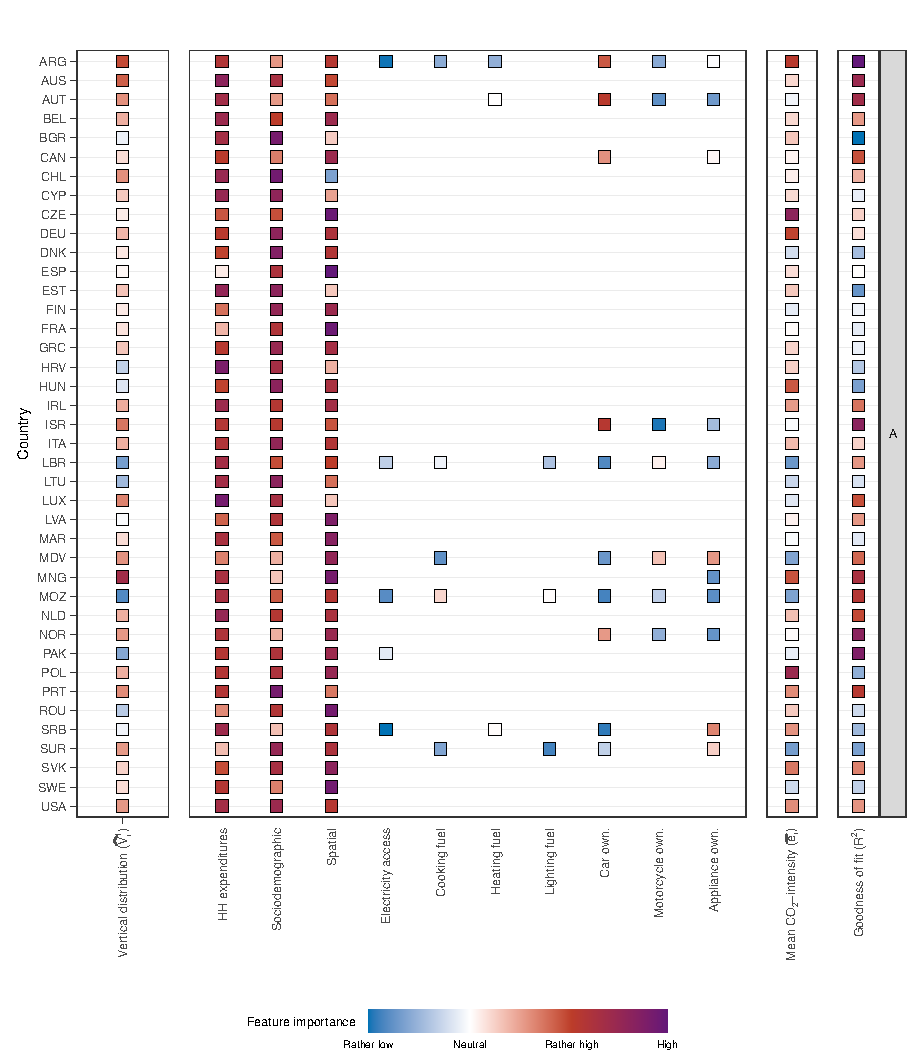
\includegraphics{1_Figures/Figure 4/Figure_4_Uncorrected_1.pdf}
     \begin{subcaption2}
    This figure shows the importance of features (in normalized average absolute SHAP-values) for each country, grouped by country clusters. Blue (red) colors indicate that a feature is relatively less (more) important in a country compared to all other countries and features. 'Sociodemographic' comprises features such as household size, gender, self-identified ethnicity, nationality, religion or language. 'Spatial' comprises features such as state, province, district and urban/rural-identifiers. For vertical distribution, blue (red) colors indicate lower (higher) median carbon intensity among the poorest quintile compared to the richest quintile. For average CO$_{2}$-intensity, blue (red) colors indicate a lower (higher) average carbon intensity across all countries. For goodness of fit (R\textsuperscript{2}), blue (red) colors indicate a lower (higher) predictive performance compared to other countries. Average CO\textsubscript{2}-intensity and R\textsuperscript{2} are not explicitly included for clustering.
    We assign countries to 12 clusters performing k-means clustering based on \textit{non-adjusted} feature importance values across all features. We also show all values in Table \ref{tab:A10_Uncorrected}.
    \end{subcaption2}
    \end{subfigure}
\end{figure}
\clearpage

\clearpage
\begin{figure}[ht!]\ContinuedFloat
    \centering
    \begin{subfigure}[b]{\textwidth}
    \centering
    \caption{Feature importance across countries of clusters D to L - non-adjusted}\label{fig:fig_4_2_uncorrected}
    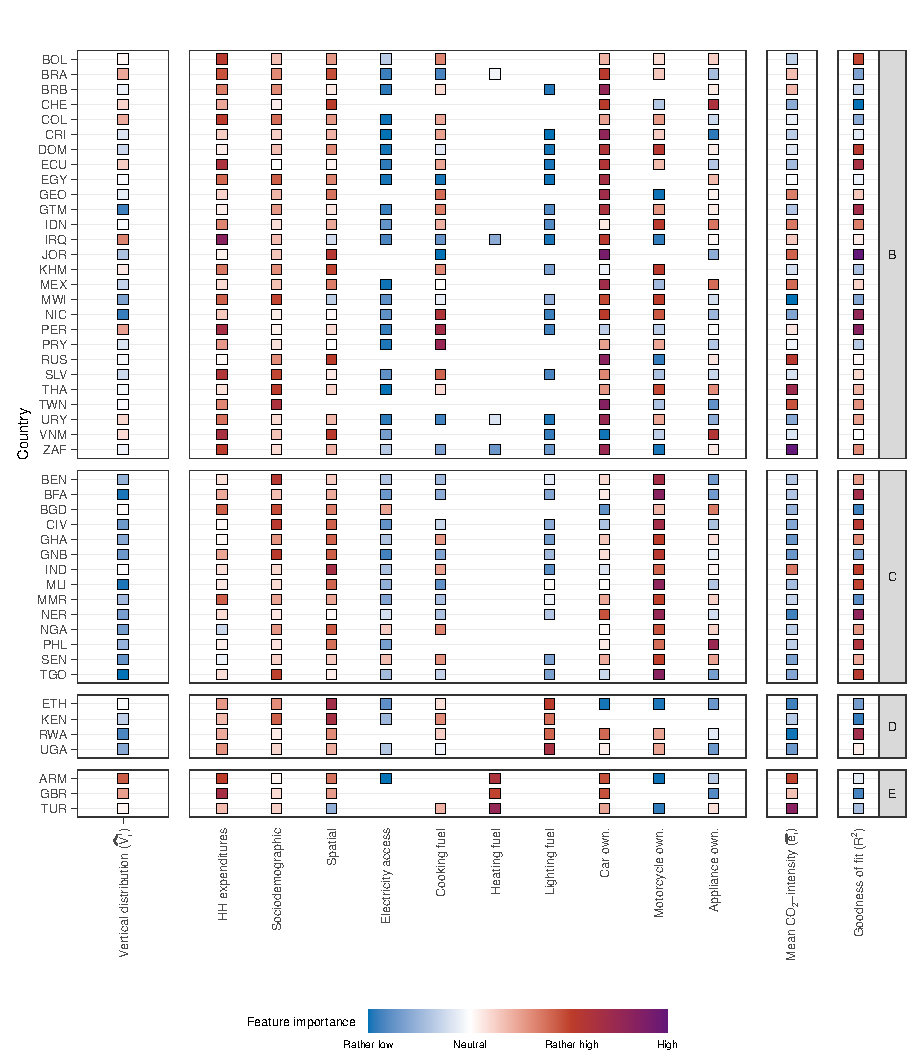
\includegraphics{Figure 4/Figure_4_Uncorrected_2.pdf}
    \begin{subcaption2}
    This figure shows the importance of features (in normalized average absolute SHAP-values) for each country, grouped by country clusters. Blue (red) colors indicate that a feature is relatively less (more) important in a country compared to all other countries and features. 'Sociodemographic' comprises features such as household size, gender, self-identified ethnicity, nationality, religion or language. 'Spatial' comprises features such as state, province, district and urban/rural-identifiers. For vertical distribution, blue (red) colors indicate lower (higher) median carbon intensity among the poorest quintile compared to the richest quintile. For average CO$_{2}$-intensity, blue (red) colors indicate a lower (higher) average carbon intensity across all countries. For goodness of fit (R\textsuperscript{2}), blue (red) colors indicate a lower (higher) predictive performance compared to other countries. Average CO\textsubscript{2}-intensity and R\textsuperscript{2} are not explicitly included for clustering.
    We assign countries to 12 clusters performing k-means clustering based on \textit{non-adjusted} feature importance values across all features. We also show all values in Table \ref{tab:A10_Uncorrected}.
    \end{subcaption2}
    \end{subfigure}
    
\end{figure}
\clearpage

\clearpage
\begin{figure}[ht!]\ContinuedFloat
    \centering
    \begin{subfigure}[b]{\textwidth}
    \centering
    \caption{Feature importance across countries of clusters A to B - imputed}\label{fig:fig_4_2_imputed}
    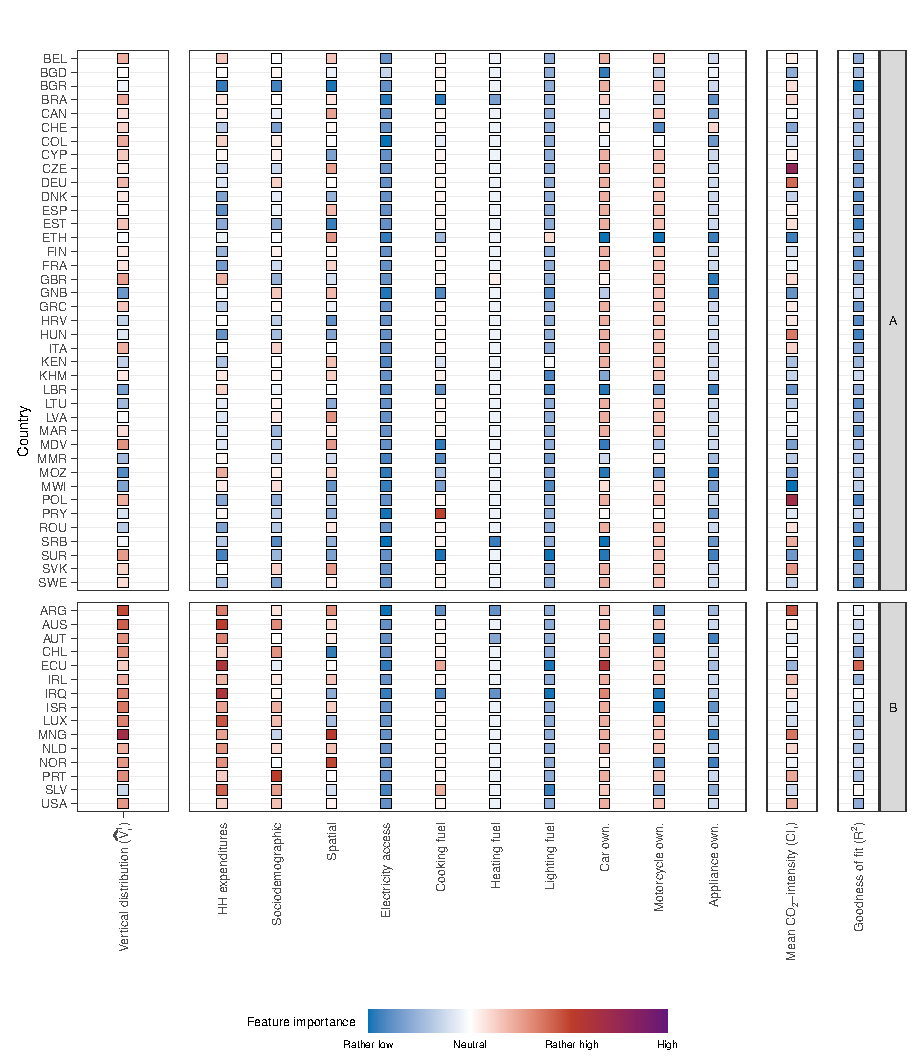
\includegraphics{Figure 4/Figure_4_Corrected_Imputed_1.pdf}
    \begin{subcaption2}
    This figure shows the importance of features (in normalized average absolute SHAP-values) for each country, grouped by country clusters. In contrast to figures \ref{fig:fig_4_1} and \ref{fig:fig_4_2}, we impute missing values for unobserved features with the average feature importance for each feature. We adjust feature importance for country-level model performance. Blue (red) colors indicate that a feature is relatively less (more) important in a country compared to all other countries and features. 'Sociodemographic' comprises features such as household size, gender, self-identified ethnicity, nationality, religion or language. 'Spatial' comprises features such as state, province, district and urban/rural-identifiers. For vertical distribution, blue (red) colors indicate lower (higher) median carbon intensity among the poorest quintile compared to the richest quintile. For average CO\textsubscript{2}-intensity, blue (red) colors indicate a lower (higher) average carbon intensity across all countries. For goodness of fit (R\textsuperscript{2}), blue (red) colors indicate a lower (higher) predictive performance compared to other countries. Average CO\textsubscript{2}-intensity and R\textsuperscript{2} are not explicitly included for clustering.
    We assign countries to 11 clusters performing k-means clustering based on \textit{adjusted} and \textit{imputed} feature importance values across all features. We also show all values in Table \ref{tab:A10_Imputed}.
    \end{subcaption2}
    \end{subfigure}
    
\end{figure}
\clearpage

\clearpage
\begin{figure}[ht!]\ContinuedFloat
    \centering
    \begin{subfigure}[b]{\textwidth}
    \centering
    \caption{Feature importance across countries of clusters C to K - imputed}\label{fig:fig_4_2_imputed}
    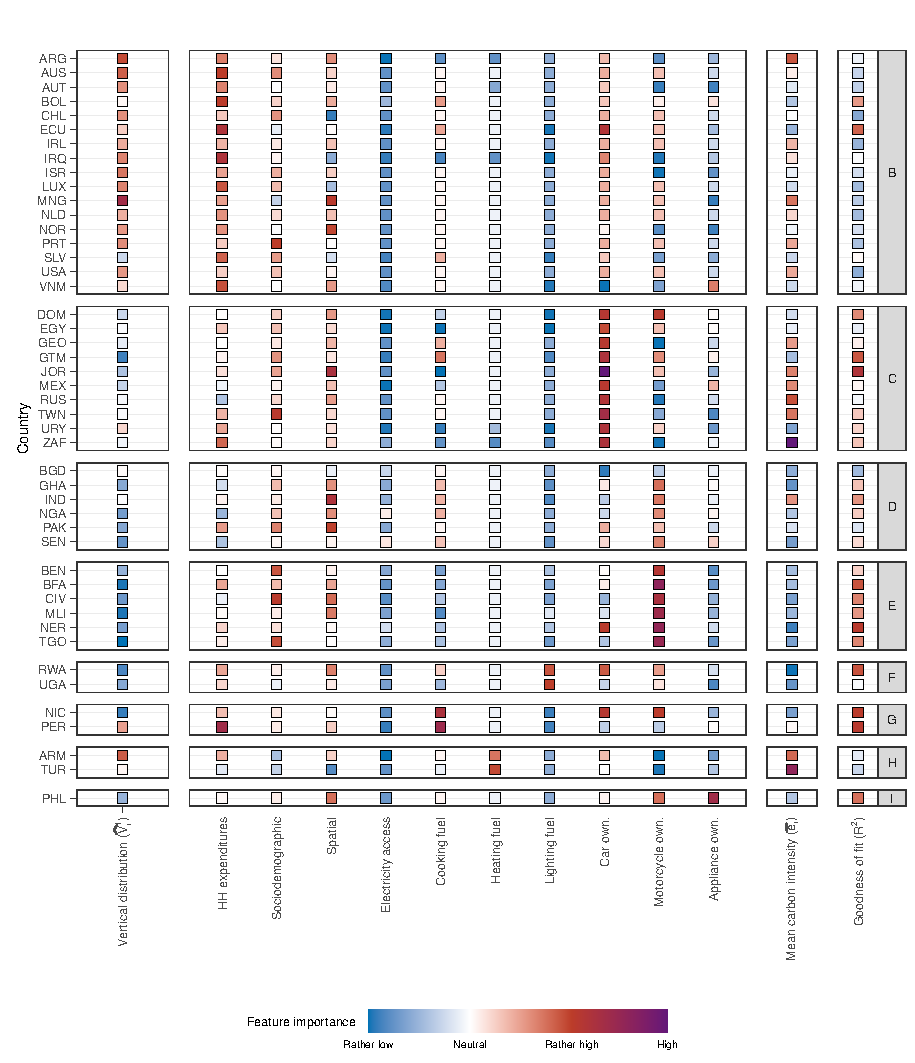
\includegraphics{Figure 4/Figure_4_Corrected_Imputed_2.pdf}
    \begin{subcaption2}
    This figure shows the importance of features (in normalized average absolute SHAP-values) for each country, grouped by country clusters. In contrast to figures \ref{fig:fig_4_1} and \ref{fig:fig_4_2}, we impute missing values for unobserved features with the average feature importance for each feature. We adjust feature importance for country-level model performance. Blue (red) colors indicate that a feature is relatively less (more) important in a country compared to all other countries and features. 'Sociodemographic' comprises features such as household size, gender, self-identified ethnicity, nationality, religion or language. 'Spatial' comprises features such as state, province, district and urban/rural-identifiers. For vertical distribution, blue (red) colors indicate lower (higher) median carbon intensity among the poorest quintile compared to the richest quintile. For average CO\textsubscript{2}-intensity, blue (red) colors indicate a lower (higher) average carbon intensity across all countries. For goodness of fit (R\textsuperscript{2}), blue (red) colors indicate a lower (higher) predictive performance compared to other countries. Average CO\textsubscript{2}-intensity and R\textsuperscript{2} are not explicitly included for clustering.
    We assign countries to 11 clusters performing k-means clustering based on \textit{adjusted} and \textit{imputed} feature importance values across all features. We also show all values in Table \ref{tab:A10_Imputed}.
    \end{subcaption2}
    \end{subfigure}
    
\end{figure}
\clearpage